\chapter{Design \& Implementation}
\label{sec:design_and_implementation}

\section{GUI}
\label{sec:gui}

The GUI consists of a menu, a two-column grid and a status bar. The features that can be interacted with in the GUI have been outlined below. An overview of the available class types can be seen on figure \ref{fig:one_each}.

\begin{figure}[htbp]
   \centering
   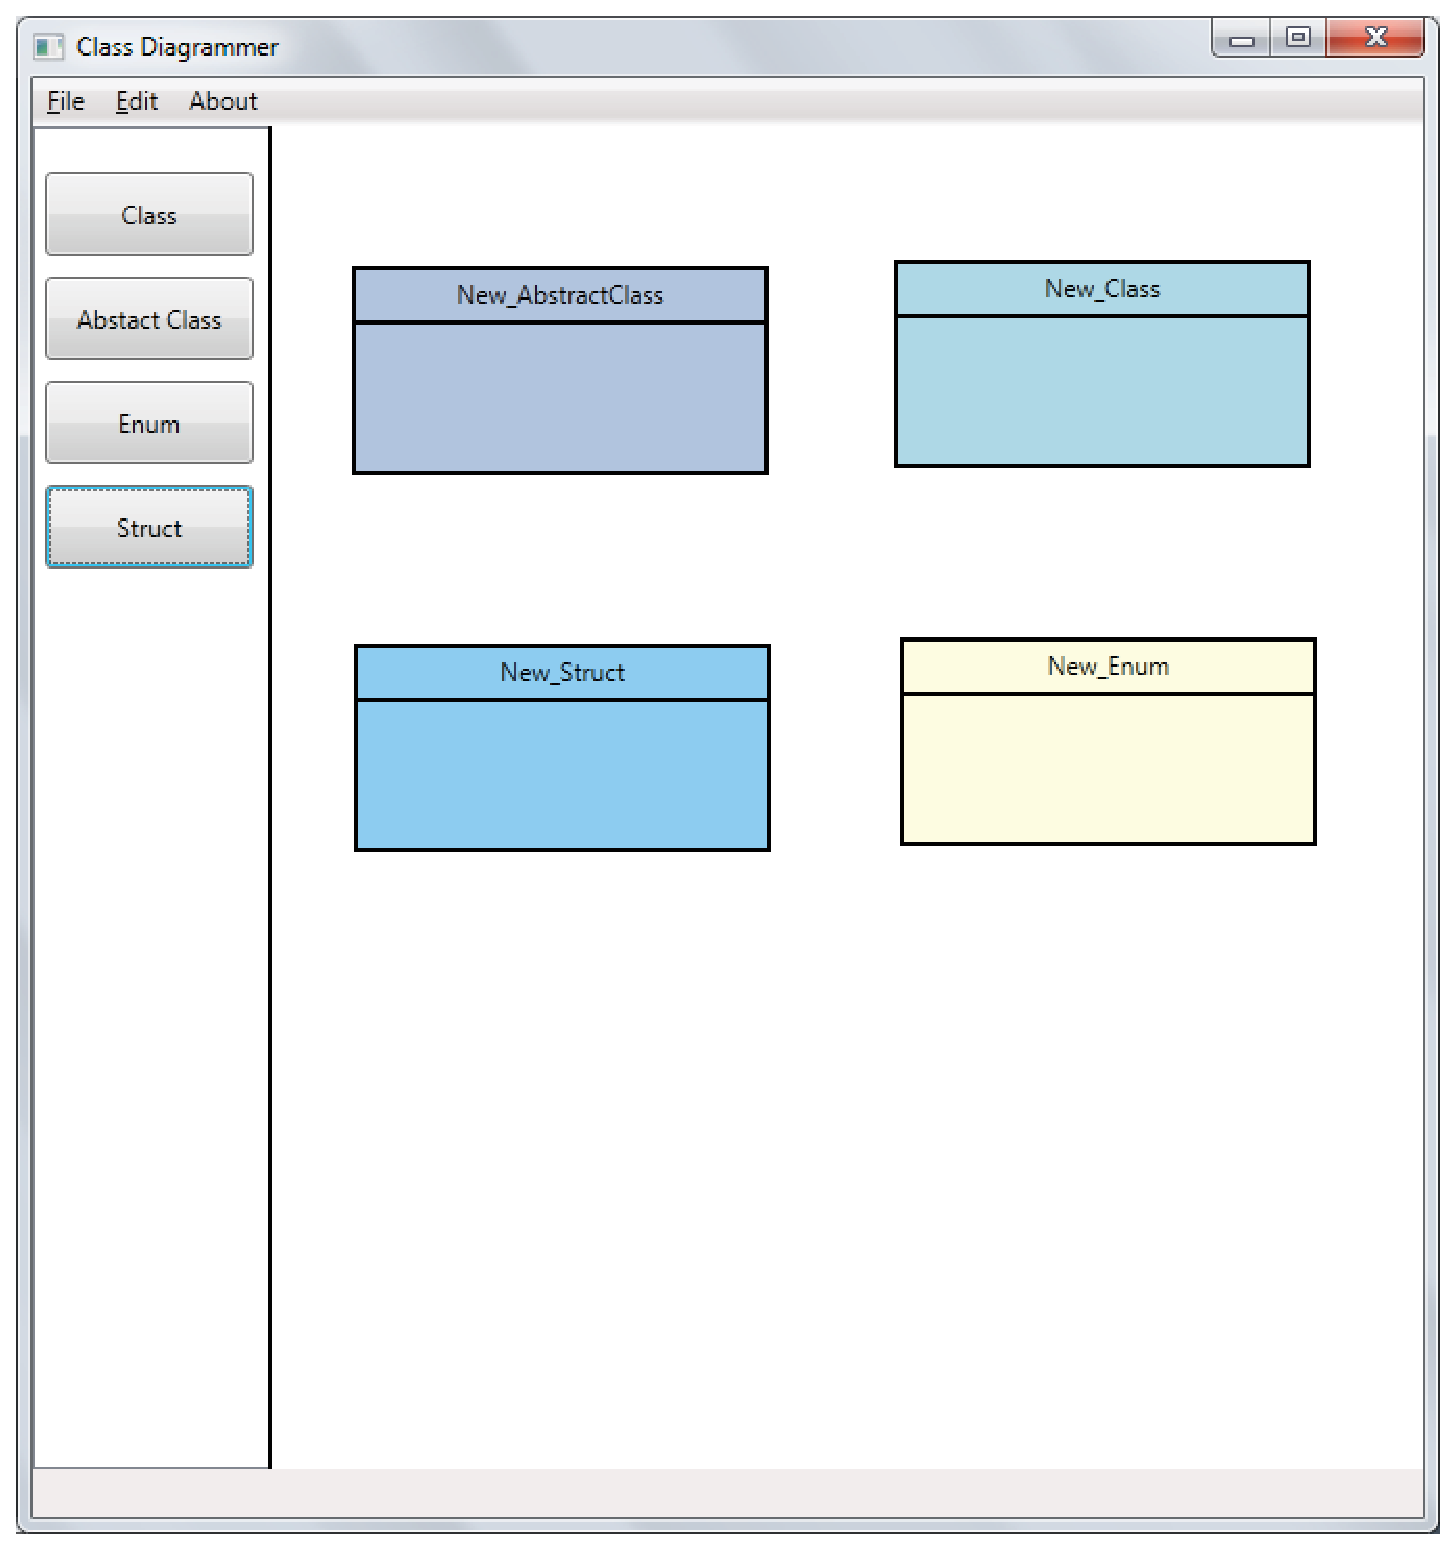
\includegraphics[width=1\linewidth]{figure/one_of_each}
   \caption{Overview of classes}
   \label{fig:one_each}
\end{figure}


\subsection{Editable classes}

There are different gestures for creating, updating and deleting classes, each chosen to get the best user experience. In the left grid column, one can click on a button to create a specific type of class in the application. At the moment there are four types to choose among:

\begin{itemize}
  \item Class
  \item Abstract Class
  \item Enum
  \item Struct
\end{itemize}

Clicking one of the buttons will also insert a box in the right grid column representing the class in the application. The color of the boxes are determined by the type of the classes.

Deleting a class is done by right clicking on the specific box representing that class.

If one wants to edit a class, this is done by double (left) clicking on the specific box. This will cause the box to switch to an editable field where one can type in the name, properties and methods for the class in accordance with the syntax of UML class diagrams. Clicking on the same box again or double clicking on another box will save the changes, and the boxes will automatically resize to fit its content. Thus, only one class can be edited at a time.

Inline text edit is chosen over a pop-up window or likewise because the UML class diagram content syntax is so simple and understandable and because it (from a programmer's point of view) is much faster to use this text based UI than pick the different properties and methods etc. in a GUI.

The parsing of inline text edit is done with regular expressions, RegEx, and is described in section \ref{sec:regex}

\begin{figure}[htbp]
   \centering
   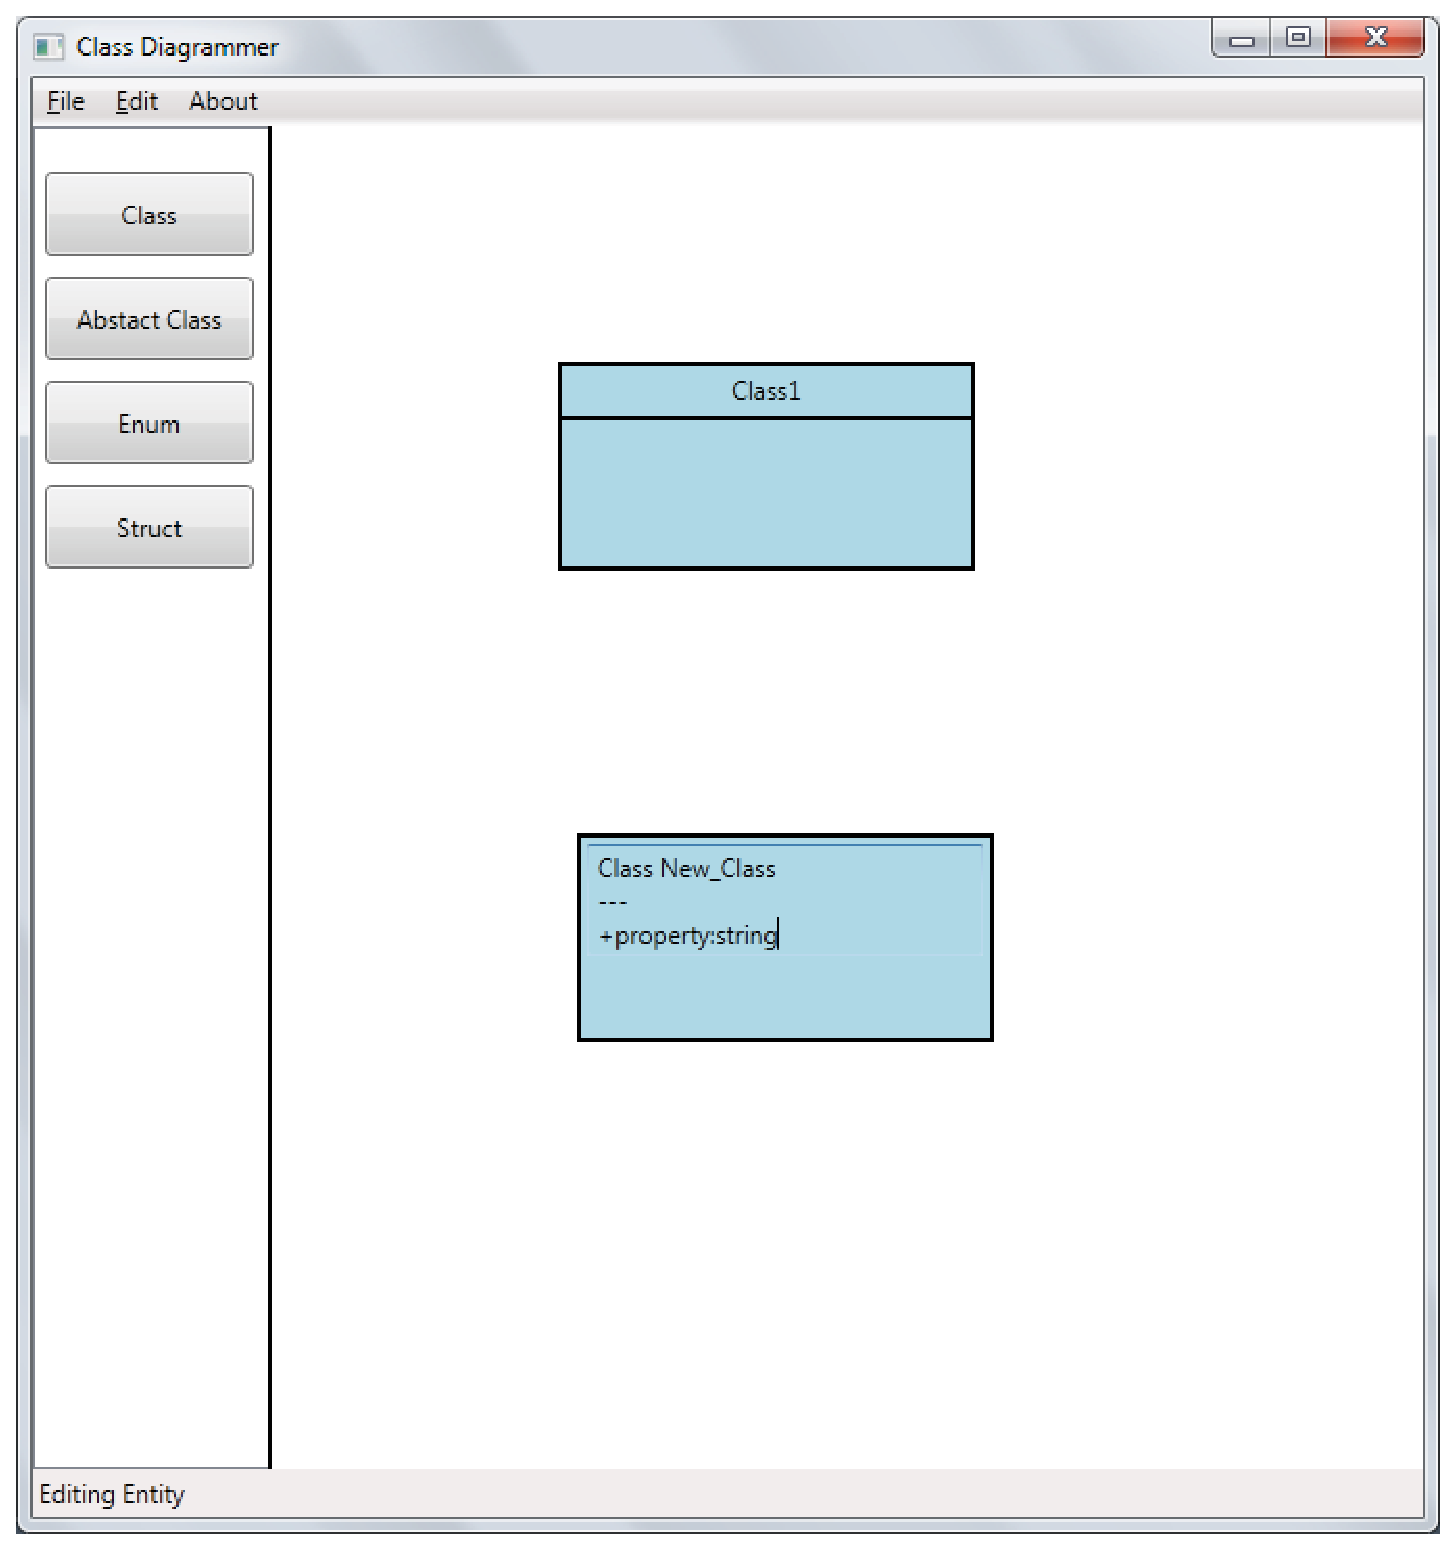
\includegraphics[width=1\linewidth]{figure/edit_text}
   \caption{Edition of a class}
   \label{fig:edit}
\end{figure}

\subsubsection{RegEx}
\label{sec:regex}
To validate and parse the text from inline edit regular expressions, or RegEx, is used. RegEx is extremely useful to parse text using defined patterns and extract parts of text.

The RegEx implemented parses the text according to the following pattern:
\begin{enumerate}
\item A visibility token\footnote{+ for public, - for private and \# for protected.}
\item A variable name
\item Optional space
\item Optional default value noted by $=$, optional space followed by the value
\item Optional space if default value specified
\item A colon ( : )
\item Optional space
\item The variables type
\item The carnality of the relation
\end{enumerate}

The RegEx parsing is done in multiple steps. The first line is the first one to be parsed against the pattern shown in listings \ref{lst:regex}. When the name and type has been parsed it checks if the second line consists of exactly three dashes ``$---$'' denoting that the rest of the lines will be either properties of functions of the class.

\begin{lstlisting}[caption={RegEx for class type and name matching},label=lst:regex]
(abstract class|class|enum|struct) (.+)
\end{lstlisting}

Each line is then matched against two patterns to see if its a function or property. If the line matches the function pattern shown in listings \ref{lst:regexfunc} the parser takes the matched groups and populates a function entry for the current class.

\begin{lstlisting}[caption={RegEx for function matching},label=lst:regexfunc]
([#+-])(.+?)\((.+)\)(?: ?: ?(.+))
\end{lstlisting}

If the line does not match the function pattern, but instead matches the property pattern as shown in listings \ref{lst:regexprop} further processing is done otherwise the line is skipped.

If a line has been successfully matched to the property pattern the type group of the pattern is then again matched against the pattern given in listings \ref{lst:regexarray} to see if it has been defined as an array.

\begin{lstlisting}[caption={RegEx for property matching},label=lst:regexprop]
([#+-])(.+?)(?: ?= ?(.+?))?(?: ?: ?(.+))
\end{lstlisting}

\begin{lstlisting}[caption={RegEx for array matching},label=lst:regexarray]
(.+?)\[([0-9]+)\]
\end{lstlisting}

The property entry is then populated with the matched groups, and if the matched type group is a name of a class already on the canvas a line is drawn between them, and the carnality is written on the line.
The carnality of the relationship is taken from the array size if specified otherwise 1 is used.

\subsection{Movable classes}
It is possible to freely move the boxes around in the right grid column, but only there. That means that it is not possible to e.g. move the boxes out of the window or into the left grid column.

When editing a box, one cannot move it, but it is still possible to move other boxes.

\subsection{Undo and redo}
The undo-redo functionality has been implemented with the command pattern.
Every time there is a change to the item canvas; add, removal or moving of classes the action is put on the undo stack.

When the undo command is then called, the stack is popped, the command is executed thus reversing the action and putting it on the redo stack. The redo command then acts in the same way as the undo command, if there is anything on the stack.

\begin{figure}[htbp]
   \centering
   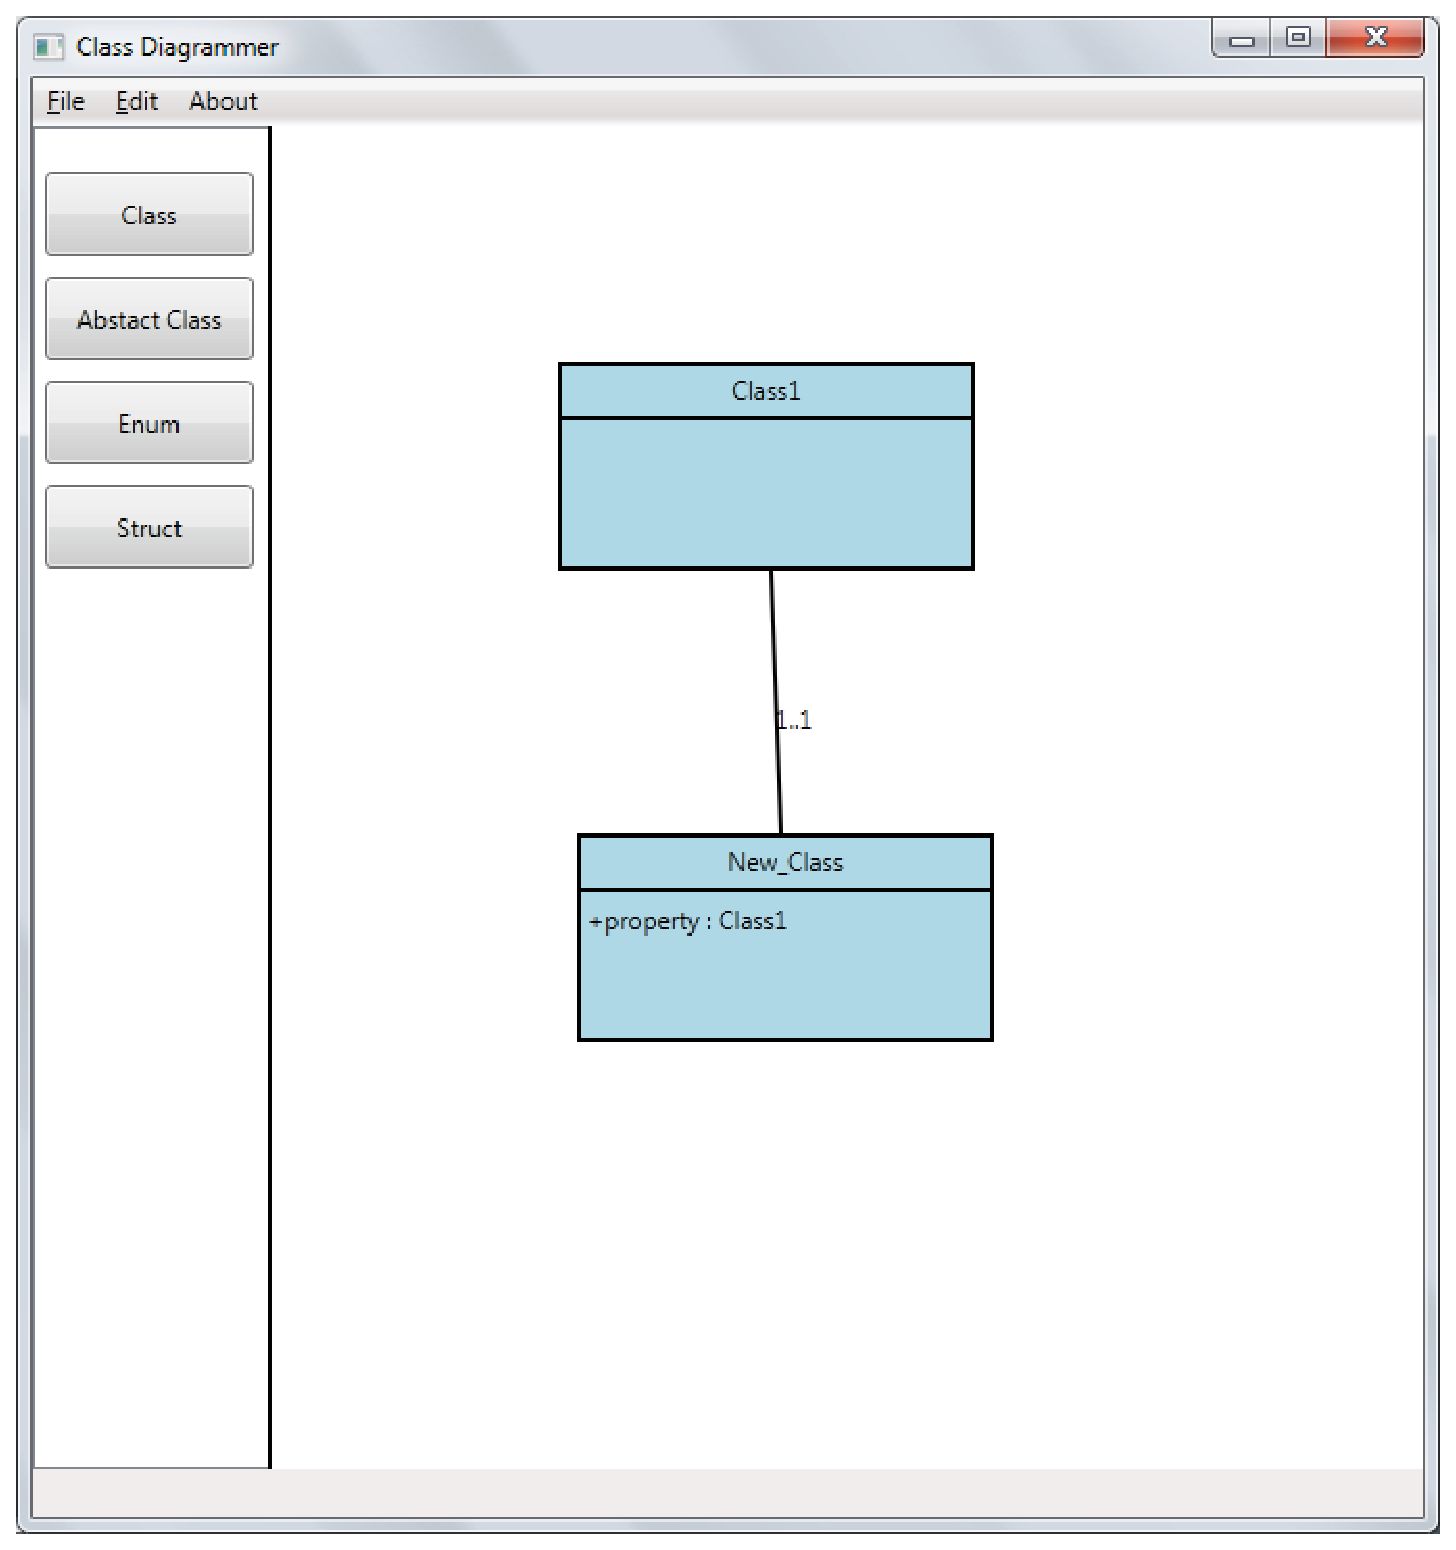
\includegraphics[width=1\linewidth]{figure/one_one_relation}
   \caption{One to one relation}
   \label{fig:one_one}
\end{figure}

\begin{figure}[htbp]
   \centering
   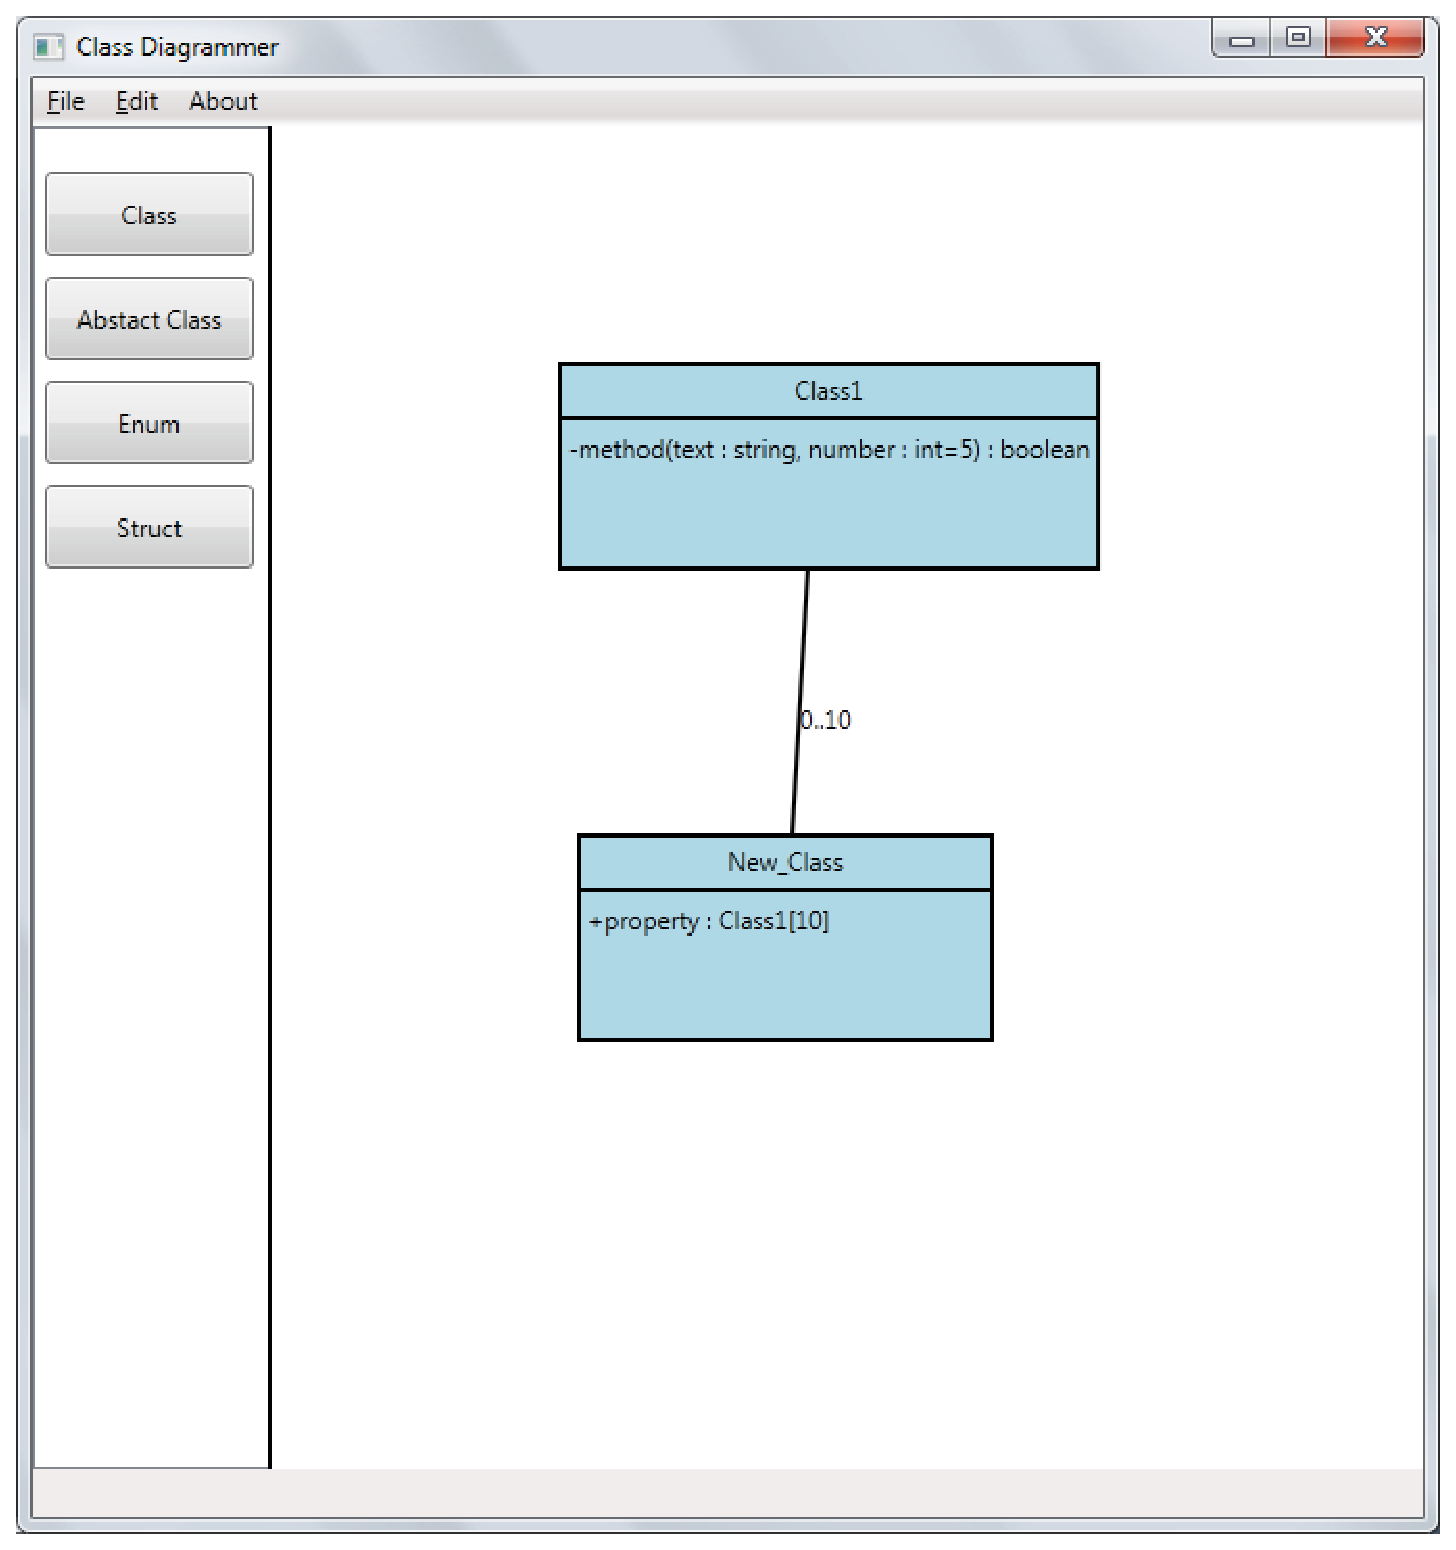
\includegraphics[width=1\linewidth]{figure/one_many_relation}
   \caption{One to many relation}
   \label{fig:one_many}
\end{figure}


\subsection{Relations}
Relations will be created, updated and deleted automatically based on the classes (boxes) present. Also, a text will say what kind of relation it is, e.g. one-to-one, one-to-many

The relationship text is depending on the information provided for the carnality as described in section \ref{sec:regex}.

\subsection{Menu and shortcuts}

In the top menu, one can find various options and functions. Each of them has been given a shortcut key combination that correspond to the default shortcut for its type (if it exists). The options and their shortcuts can be seen in table \ref{tab:menu_shortcut}.

\begin{table}[htbp]
\centering
\begin{tabular}{|l|l|}
\hline
\textbf{Option} & \textbf{Shortcut}\\
\hline
New file & Ctrl+N\\
\hline
Open file & Ctrl+O\\
\hline
Save file & Ctrl+S\\
\hline
Save as & Ctrl+A\\
\hline
Undo & Ctrl+Z\\
\hline
Redo & Ctrl+Y\\
\hline
\end{tabular}
\caption{Shortcuts of menu options}
\label{tab:menu_shortcut}
\end{table}

\subsection{Status bar}

On the bottom of the GUI a status bar can be seen. Here, the user gets messages about what the status is, i.e. what is going on in the application. E.g. if a box is being edited, removed, moved or if a file is being (automatically) saved or loaded.

\section{Application layer}
\label{sec:app_layer}

\subsection{DLL}
To ensure the application is extensible all models have been put in a separate DLL file.

This way, the model layer can be reused in another application or context, e.g.  a web based UML diagram application.

\subsection{Save and load}
The save functionality has been implemented in its own thread, because the application could otherwise be halted while this operation were executed. The load functionality remains in the same thread as the GUI, because one should not be able to modify the canvas while loading a file.

A prettier solution would be to use background workers to load the file meanwhile the GUI was disabled or perhaps showing a progress bar. When the background workers had completed loading the GUI was to be enabled again.

After a file has been saved the first time, the application will automatically save it continuously in a specific time interval. This way, the user does not have to worry about losing hours of work if the computer crashes or shuts down.

The application saves the applications state by taking the list of classes on the canvas (\textsf{List<Base>} in the source code) and serializing the entire list with a binary formatter whose output is then saved to a file on the computer.

\section{Design patterns}
\label{sec:design_pattern}
\subsection{Singleton}
The singleton design pattern restricts the instantiation of a class to one object.
The pattern is useful when exactly one object is needed to coordinate actions or use of data throughout the system, such as a config class or data model.

The singleton pattern is implemented in the \textsf{Serializer} class, that is used when saving and loading files. 

The singleton pattern is also used by the MVVM framework GallaSoft for interacting with the \textsf{MainViewModel} to ensure, that it is the same instance of the class that is being used throughout the application, thus the same data.

\subsection{Command}
The command pattern is a behavioural design pattern where an object is used to encapsulate all information needed to call a method at a later time.
The command pattern is useful for implementing GUI button, undo/redo, wizards and transactional behavior.

The command pattern has been used to implement the undo-redo feature.

\subsection{MVVM}
The Model View ViewModel is an architechtural design pattern used in software development. It originated from Microsoft and was introduced by Martin Fowler.
MVVM is targeted at modern UI development platforms which supports event-driven programming such as Windows Presentation Foundation, Silverlight and HTML5.
MVVM is largely based on the Model View Controller, MVC, pattern which strives to separate presentation logic from business logic and data.

MVVM has the same data separation as MVC, as it uses a ViewModel to expose the data from the data model to the view for presentation.
The pattern was designed to make use of the data binding functions of WPF, which would facilitate the separation of the view layer development
from the rest of the pattern thus removing almost all GUI code from the view layer.

Instead of the user interface developers to write GUI code, it is possible for them to use markup language instead (such as XAML)
and create data bindings to the ViewModel, which is made by the application developers.

This seperation allows for higher productivity because application and UX developers are working on different parts of the program, 
without them having to worry about the other party's code.
Even if the application is developed by a single developer, said developer would still benefit from this separation of logic 
in the late development cycles where the UI often changes frequently based on end-user feedback.

\section{Tests}
\label{sec:tests}
Throughout the development of the application several tests has been conducted to ensure that the application is performing as expected.

The various use cases used for testing the application can be found in appendix \ref{ap:usecase}.